\section{Model Based Approach}
\label{sec:modelbased}
Based on the insights described in the previous section, we will propose a model for SQL-on-Hadoop engines. We will show that even though the model is simple, it is a sufficient approximation to generate to good recommendations. 

The inputs to the algorithms are:
\begin{enumerate}
    \item[$\bullet$] Optimization Function  
    \item[$\bullet$] Job Parameters: These are the key input parameters of the job that effect performance and cost. Table \ref{table:job_params} defines these job parameters.
    \item[$\bullet$] Instance configuration: Table \ref{table:inst_conf} defines the machine configuration.
    \item[$\bullet$] Global Parameters: These are some of the global parameters that can be used to tune the algorithm. These are defined in Table \ref{table:global_params}.
\end{enumerate}

Algorithm \ref{jobfit} optimizes resource utilization of a SQL query. 

\renewcommand{\algorithmicrequire}{\textbf{Input:}}
\renewcommand{\algorithmicensure}{\textbf{Output:}}
\renewcommand{\algorithmiccomment}[1]{// #1}
\begin{algorithm}
\caption{fitJob}\label{jobfit}
\begin{algorithmic}[1]
\footnotesize
\REQUIRE  $\mathcal{P}$ is the job parameters (defined in table \ref{table:job_params} ) to be recommended, $I_{old}$  is instance configuration (defined in Table \ref{table:inst_conf}) on which $\mathcal{P}$ is collected, $I_{new}$ is new instance configuration on which $\mathcal{P}$ needs to be optimized upon, $\mathcal{G}$ is the global parameters defined in Table \ref{table:global_params}
\ENSURE New Job parameter $\mathcal{P}_{new}$ that optimize the cumulative time of containers.
\STATE newMemPerCore $\gets I_{new}$.nodeMemory $/ I_{new}$.vCpuPerNode
\STATE $\mathcal{P}_{new}$.mapperMemory $\gets newMemPerCore$
\STATE $\mathcal{P}_{new}$.reducerMemory $\gets newMemPerCore$
\STATE ioSort $\gets$ newMemPerCore $\times$ ioSortFrac
\IF {ioSort $>$ $\mathcal{G}$.maxIOSort}
\STATE ioSort $\gets$ $\mathcal{G}$.maxIOSort
\ENDIF
\STATE $\mathcal{P}_{new}$.ioSort $\gets$ ioSort
\STATE outPerMap $\gets$ $\mathcal{P}$.mapperOutputBytes $/$ $\mathcal{P}$.numOfMapper
\STATE newSplitSize $\gets$ $\mathcal{P}$.splitSize $\times$ ioSort $/$ outPerMap
\STATE $\mathcal{P}_{new}$.splitSize $\gets$ newSplitSize
\STATE newBPR $\gets$ ($\mathcal{P}$.reducerMemory $\times$ $\mathcal{P}$.mapperInputBytes) $/$ ($\mathcal{P}$.mapperOutputBytes $\times$ $\mathcal{G}$.reducerFrac)  
\STATE $\mathcal{P}_{new}$.bytesPerReducer $\gets$ newBPR
\STATE \RETURN $\mathcal{P}_{new}$
\end{algorithmic}
\end{algorithm}

%\begin{algorithm}
%\caption{checkFit} \label{checkfit}
%\begin{algorithmic}[1]
%\footnotesize
%\REQUIRE $\mathcal{P}$ is the job parameters (defined in \ref{table:job_params} ), $\mathcal{I}$  is instance configuration (defined in \ref{table:inst_conf})
%\ENSURE Returns \textit{true} if $\mathcal{P}$ can fit into $\mathcal{I}$, otherwise \textit{false}.
%
%\STATE newMemPerCore $\gets \mathcal{I}.nodeMemory / \mathcal{I}.vCpuPerNode$
%\IF {newMemPerCore $> \mathcal{P}.mapperMemory$ and newMemPerCore $> \mathcal{P}.reducerMemory$}
%\RETURN \textit{true}
%\ELSE
%\RETURN \textit{false}
%\ENDIF
%\end{algorithmic}
%\end{algorithm}

\subsection{Results}
We evaluated the effectiveness of model based method by running experiments on real workloads. The experiments were carried out for a HIVE on MR engine. To quantify the prediction error by the model, we ran an experiment on 4 queries of a customer. Figure \ref{fig:modelbasedresult} shows the benefit predicted by our model and the actual observed benefit for these queries. The actual savings closely match the predicted savings indicating that the model is sufficiently accurate.

\begin{figure}[h]
	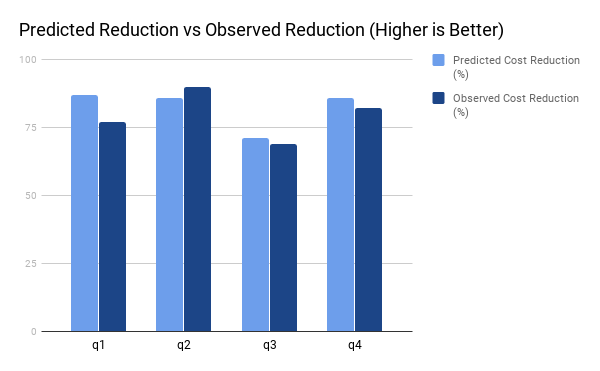
\includegraphics[width=\linewidth]{chart.png}
	%\vspace*{-15pt}
	\caption{Model Based Result: Predicted reduction in cost versus Actual reduction in cost}
	\label{fig:modelbasedresult}
\end{figure}
